\section{Konzept}

\subsection{Kontextdiagramm}
\begin{figure}[H]
  \begin{center}
    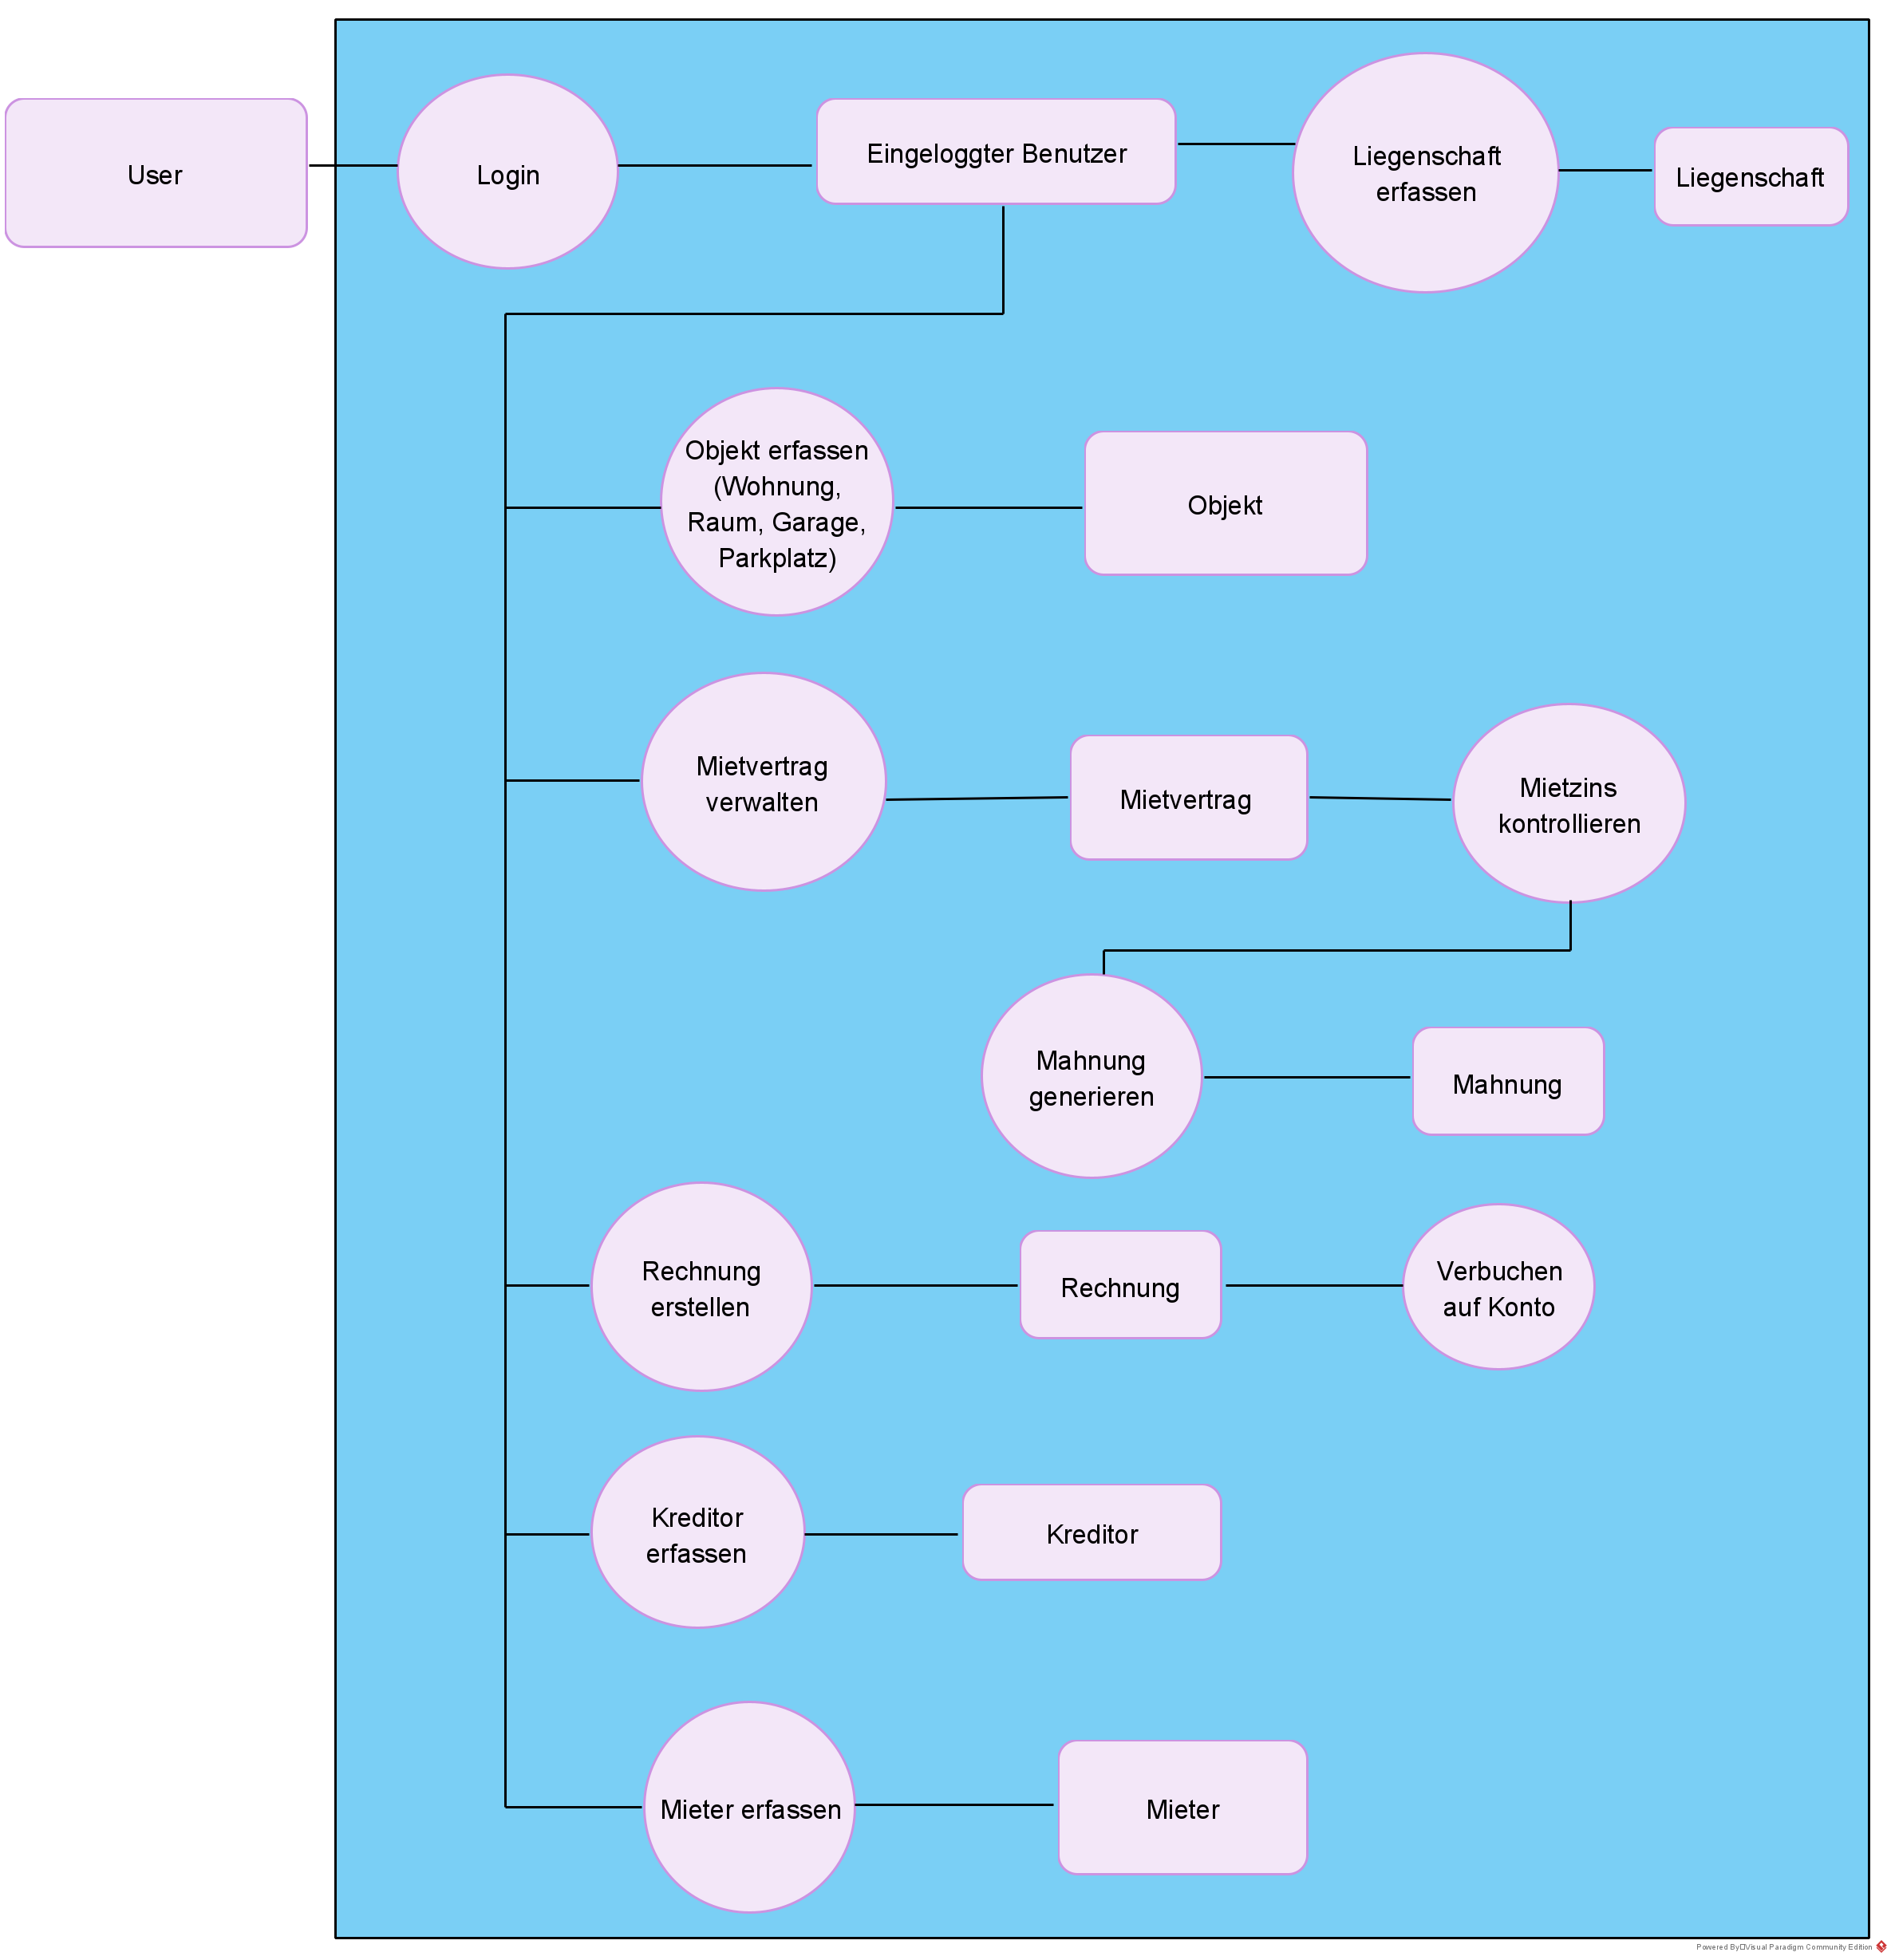
\includegraphics[width=0.99\linewidth]{content/diagrams/out/contextdiagram/context.png}
    \caption{Kontextdiagramm}
  \end{center}
\end{figure}

\subsection{Geschäftsprozessanalyse}
\subsection{Detailanforderungen an das neue System}
\subsubsection{Funktionale Anforderungen}
\begin{table}[h]
  \centering
  \settowidth\tymin{\textbf{Prio}}
  \setlength\extrarowheight{2pt}
  \begin{tabulary}{1.0\textwidth}{|L|L|}
    \hline
    \textbf{Übersicht der Mietobjekte}&\textbf{Prio}\\
    \hline
    Dem Benutzer muss beim öffnen der Applikation eine Übersicht der Mitobjekte zur verfügung stehen. Es wird pro Objekt angezeigt, ob das Objekt vermietet ist oder nicht. & 1\\ 
    \hline
  \end{tabulary}
  \caption{AF-1.1}
  \label{af1.1}
\end{table}

\begin{table}[h]
  \centering
  \settowidth\tymin{\textbf{Prio}}
  \setlength\extrarowheight{2pt}
  \begin{tabulary}{1.0\textwidth}{|L|L|}
    \hline
    \textbf{Mietverträge}&\textbf{Prio}\\
    \hline
    Die Applikation muss die Mietverträge verwalten können und die in den Musskriterien beschriebenen Angaben verwalten können. & 1\\ 
    \hline
  \end{tabulary}
  \caption{AF-1.2}
  \label{af12}
\end{table}

\subsubsection{Nichtfunktionale Anforderungen}
\subsubsection{Organisatorische Anforderungen}

\subsection{Use-Case-Beschreibungen}
\subsection{Sequenzdiagramme}
\subsection{Modellierung der Klassen}
\begin{figure}[H]
  \begin{center}
    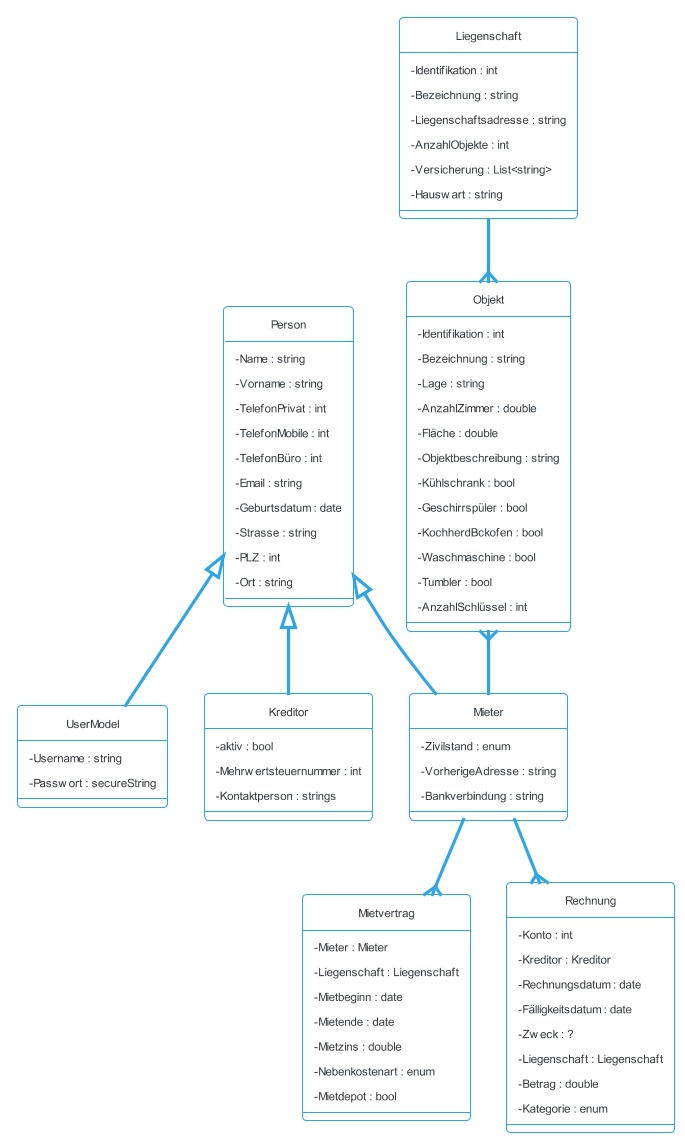
\includegraphics[width=0.75\linewidth]{content/diagrams/out/classdiagramm/ImmoGlobal.png}
    \caption{Klassendiagramm}
  \end{center}
\end{figure}

\subsection{Zustandsdiagramme}
\subsection{Modellierunge der Datenbank}
\subsubsection{ERD}
\subsubsection{Beschreibung der Fachentitäten, Beziehungen und der referenziellen Integritätsbedingungen}
\subsection{Systemarchitektur}
\subsection{Testkonzept}
\subsubsection{Vorgehen}
\subsubsection{Testobjekte}
\subsubsection{Testfälle}
\subsection{Einführungskonzept}
\subsection{GUI-Design}
